All SimCenter applications are available at the \href{https://simcenter.designsafe-ci.org/research-tools/overview/}{SimCenter website} under \emph{Research Tools}. The following sections outline the steps necessary to download and install the  \thisSoftware  application. The SimCenter applications do require that you install a number of other applications that are needed to run the workflows on your local machine as well as at DesignSafe. \\


%===============================================================================
\section{Download the Application}
%===============================================================================

% \subsection{Download the Application Files}

To download the EE-UQ application navigate to the \href{\thisSoftwarePage}{\thisSoftware page}  and click on the \emph{Download App \& User Manual} link on the right side of the page. This will bring you to another page which, as shown in \autoref{fig:app_choose_file},  contains a list of files and directories. 


\begin{figure}[!htbp]
  \centering {
    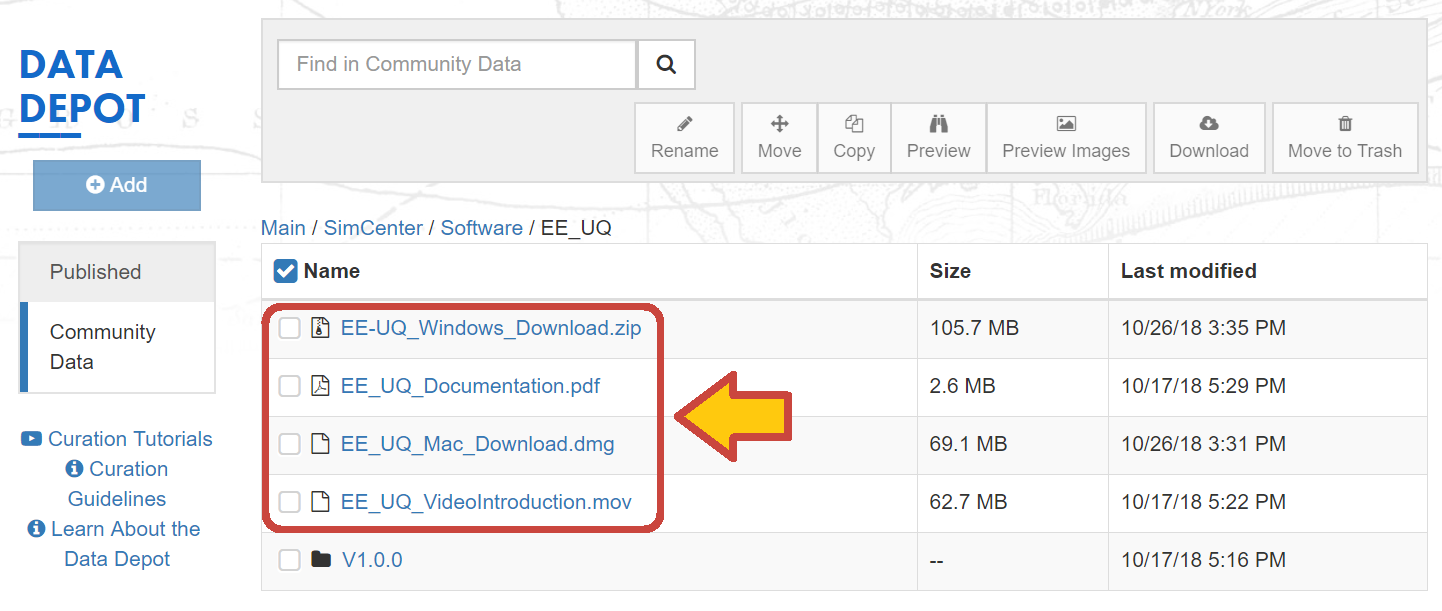
\includegraphics[width=0.8\textwidth]
    {figs/install/EE-UQ_app_choose_file.png} }
  \caption{SimCenter Tool Download Page}
  \label{fig:app_choose_file}
\end{figure}

There are at least four files available for download from this page: 
\begin{enumerate}
    \item The PDF file is the User Manual that you are reading now.
    \item The MOV file is an video that provides an introduction to the usage of the application.
    \item The ZIP file is an archive that contains the application files for a Windows operating system.
    \item The DMG file is an archive that contains the application files for a Mac OS X operating system.
\end{enumerate}

To download the \thisSoftware application click on the link for the appropriate file for your operating system  and then click on the Download button at bottom right corner of the ensuing pop-up window to download it. You need to unpackage the application from the downloaded file and place it in a location on your filesystem. On Windows, we recommend you to create a \texttt{C:/SimCenter/EE-UQ} directory and extract the contents of the \texttt{ZIP} archive there. On Mac, we recommend you to put the application in either your Documents folder or your Desktop folder. You are free to place the applications anywhere you wish, you will just need to make the appropriate adjustments with the following instructions if you do. \\

Now quickly test that the application starts. To do this navigate to the location where you placed the application and open it. You should see the user interface (UI) shown in  \autoref{fig:app_UI} after starting the application.\\

\begin{figure}[!htbp]
  \centering {
    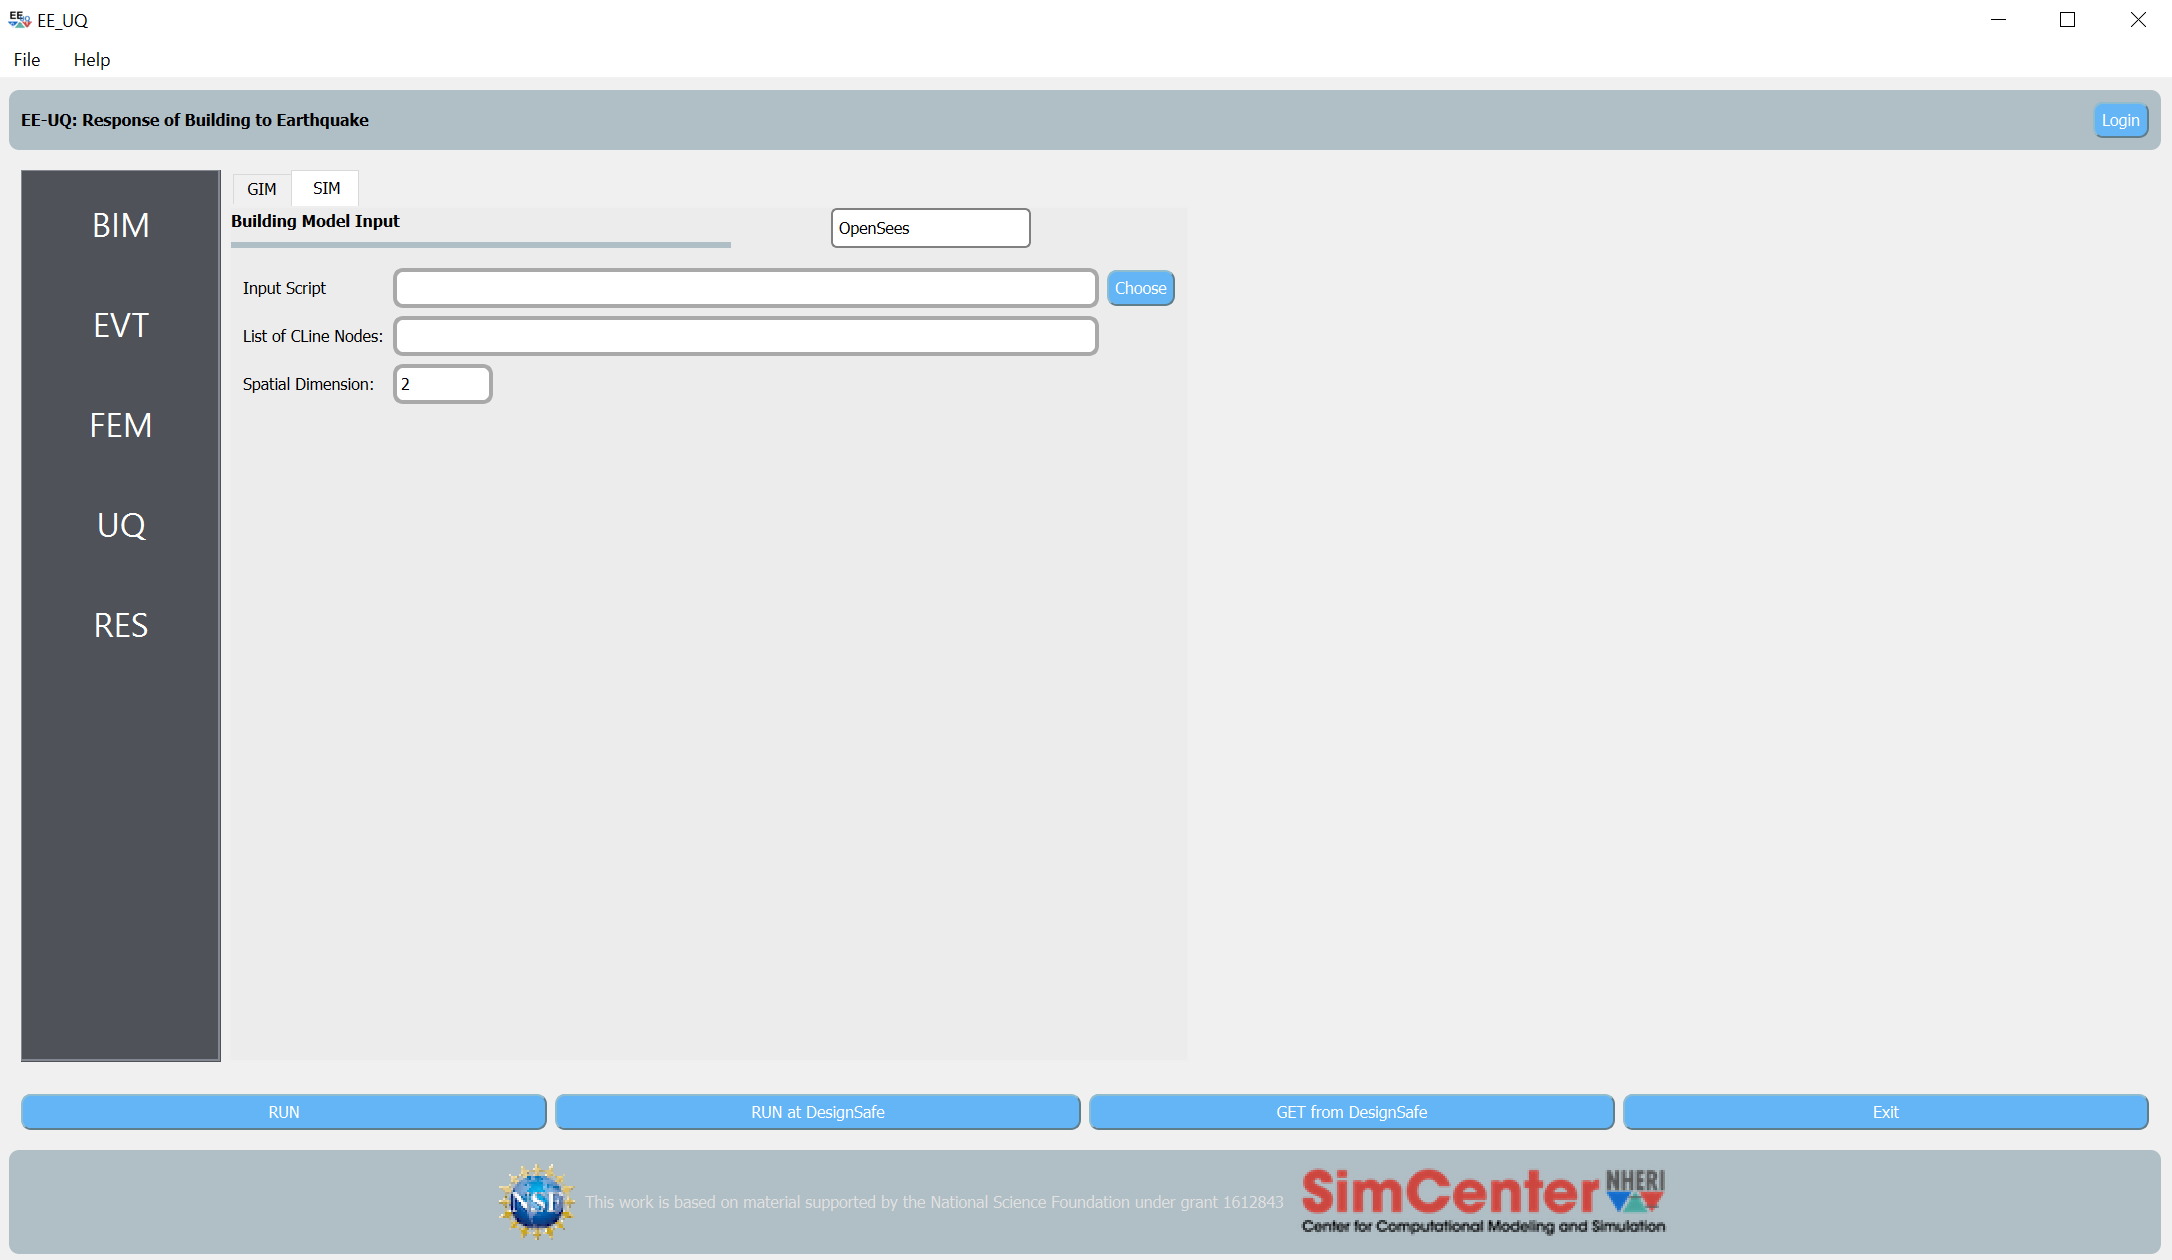
\includegraphics[width=0.8\textwidth]
    {figs/install/EE-UQ_app_UI.png} }
  \caption{The EE-UQ user interface after loading the application.}
  \label{fig:app_UI}
\end{figure}

Notes: 
\begin{enumerate}
\item The SimCenter is not recognized as either a Windows or an Apple vendor. Our applications are not recognized by the operating system as being signed. Consequently, you may receive a warning message when you start the EE-UQ application for the first time.
\item  On a Mac you will need to right click on the .dmg file to open it. Furthermore, the UI will not start correctly while in the DMG file, you need to open the .dmg file and then copy the \thisSoftware application to your Documents or Desktop folder. You can then move the .dmg file to the trash or eject it after this has been done.
\item  The \thisSoftware application requires additional software to work properly. Although the user interface loads, you will not be able to run calculations before installing those software.
\end{enumerate}



%===============================================================================
\section{Set up Python}
%===============================================================================

The SimCenter workflow applications are managed by Python scripts. These are required to prepare the input data for running analyses remotely on DesignSafe and also required for running simulations locally. As a consequence the user must have Python installed on their machine and have the appropriate environment variables set so that the UI can run these applications.

\subsection{Install Python}

If you do not have a Python installation yet, we recommend installing \href{http://www.anaconda.com/distribution/#download-section}{Anaconda}. Anaconda provides all the important scientific packages in a single convenient install. We recommend installing the 64-Bit version based on Python 3.5 or newer.

Note: If you already have a Python installation that is Python 2.7 or newer, you do not have to install Anaconda to work with SimCenter applications. You may also use another Python distribution. However, if you do  please make sure that you install the following packages available: \texttt{numpy}, \texttt{scipy}, \texttt{pandas}.

\subsection{Test Python}
%===============================================================================

Test if the python environment is set up properly by executing \texttt{python} in a terminal window. After Python starts, test if the packages are installed by executing \texttt{import numpy}, \texttt{import scipy}, and \texttt{import pandas}. You will receive an error message if a pacakage is missing. If no error appears, the terminal should look similar to \autoref{fig:python_test}. Exit Python by executing the \texttt{exit()} command.

\begin{figure}[!htbp]
  \centering {
    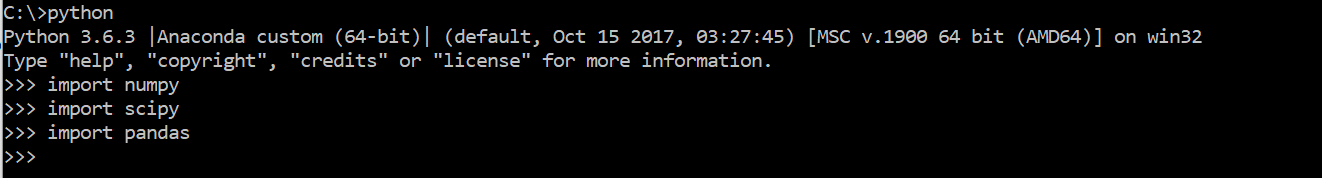
\includegraphics[width=0.8\textwidth]
    {figs/install/python_test.png} }
  \caption{Testing the Python environment.}
  \label{fig:python_test}
\end{figure}

%===============================================================================
\section{Set up for Running Workflows Locally}\label{setup}
%===============================================================================

To run the workflows locally, the backend python application needs publicly available software to also be installed on your machine. These software applications need to be installed and configured on your operating system. If you do not plan to run the workflows locally, you will not need these applications.

\subsection{Install OpenSees}
%===============================================================================

\href{https://opensees.berkeley.edu}{OpenSees} is an open-source finite element application publicly available for download from its \href{https://opensees.berkeley.edu/OpenSees/user/download.php}{download page}. If you have never downloaded OpenSees you will need to register your e-mail to gain access. After registration, you can proceed to the download page. OpenSees installation requires the user install both OpenSees and Tcl. The Windows and Mac downloads are in different locations on the download page, with the appropriate tcl installer beside the OpenSees link as is shown in \autoref{fig:opensees_installation}

\begin{figure}[!htbp]
  \centering {
    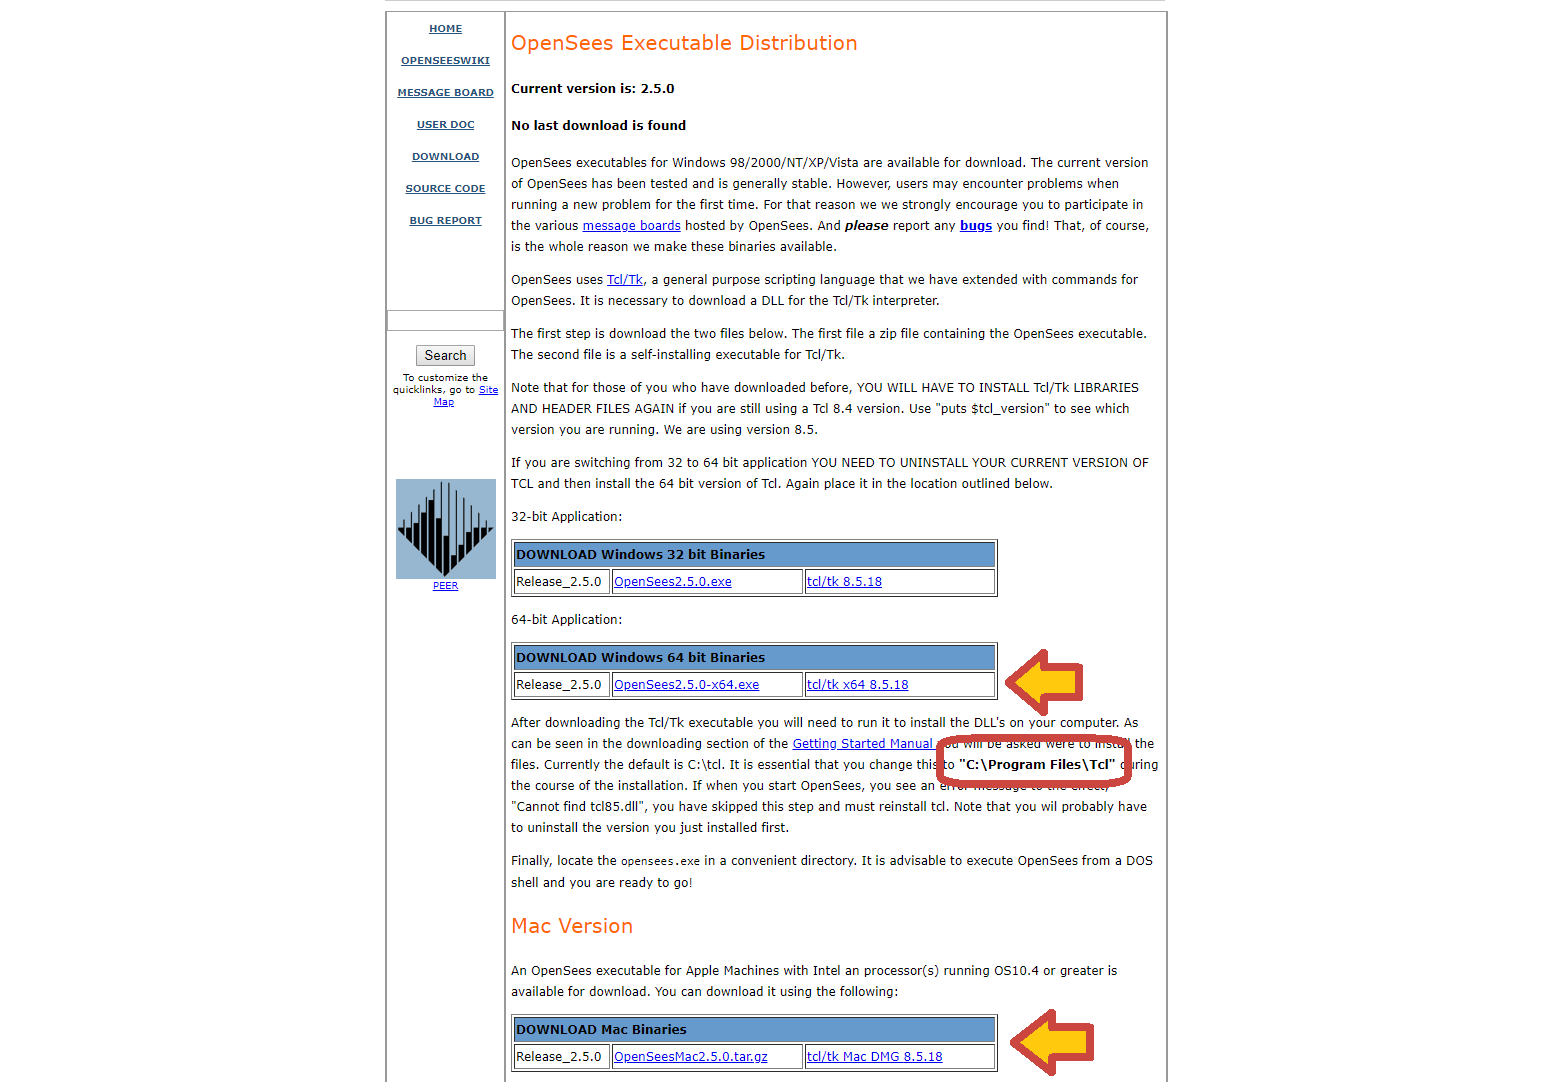
\includegraphics[width=0.8\textwidth]
    {figs/install/opensees_installation.png} }
  \caption{Installation instructions for OpenSees.}
  \label{fig:opensees_installation}
\end{figure}

Follow the instructions on this page to install Tcl (\autoref{fig:opensees_installation}). On Windows, pay particular attetion to the location Tcl must be installed in, as this is not the default, and make sure you run the installer as administrator, otherwise you will not be able to create the \texttt{C:/Program Files/Tcl} folder.

After Tcl is installed, we recommend you put OpenSees in the \texttt{C:/SimCenter/OpenSees} folder on Windows and in a \texttt{/usr/local/OpenSees} directory on the Mac (If you use finder on Mac to do navigation, use command-shift-G in Finder and specify /usr/local as the folder to go to. There create a new folder OpenSees and copy the OpenSees application to this folder).\\


Now  you need to add the \texttt{OpenSees} folder to the system \texttt{PATH} environment variable to allow the SimCenter workflow applications to find the OpenSees executable on your computer. The steps to do this depend on your operating system:

\begin{enumerate}
\item Windows: To add a folder to the \texttt{PATH} on Windows (\autoref{fig:add_env_path}):

\begin{figure}[!htbp]
  \centering {
    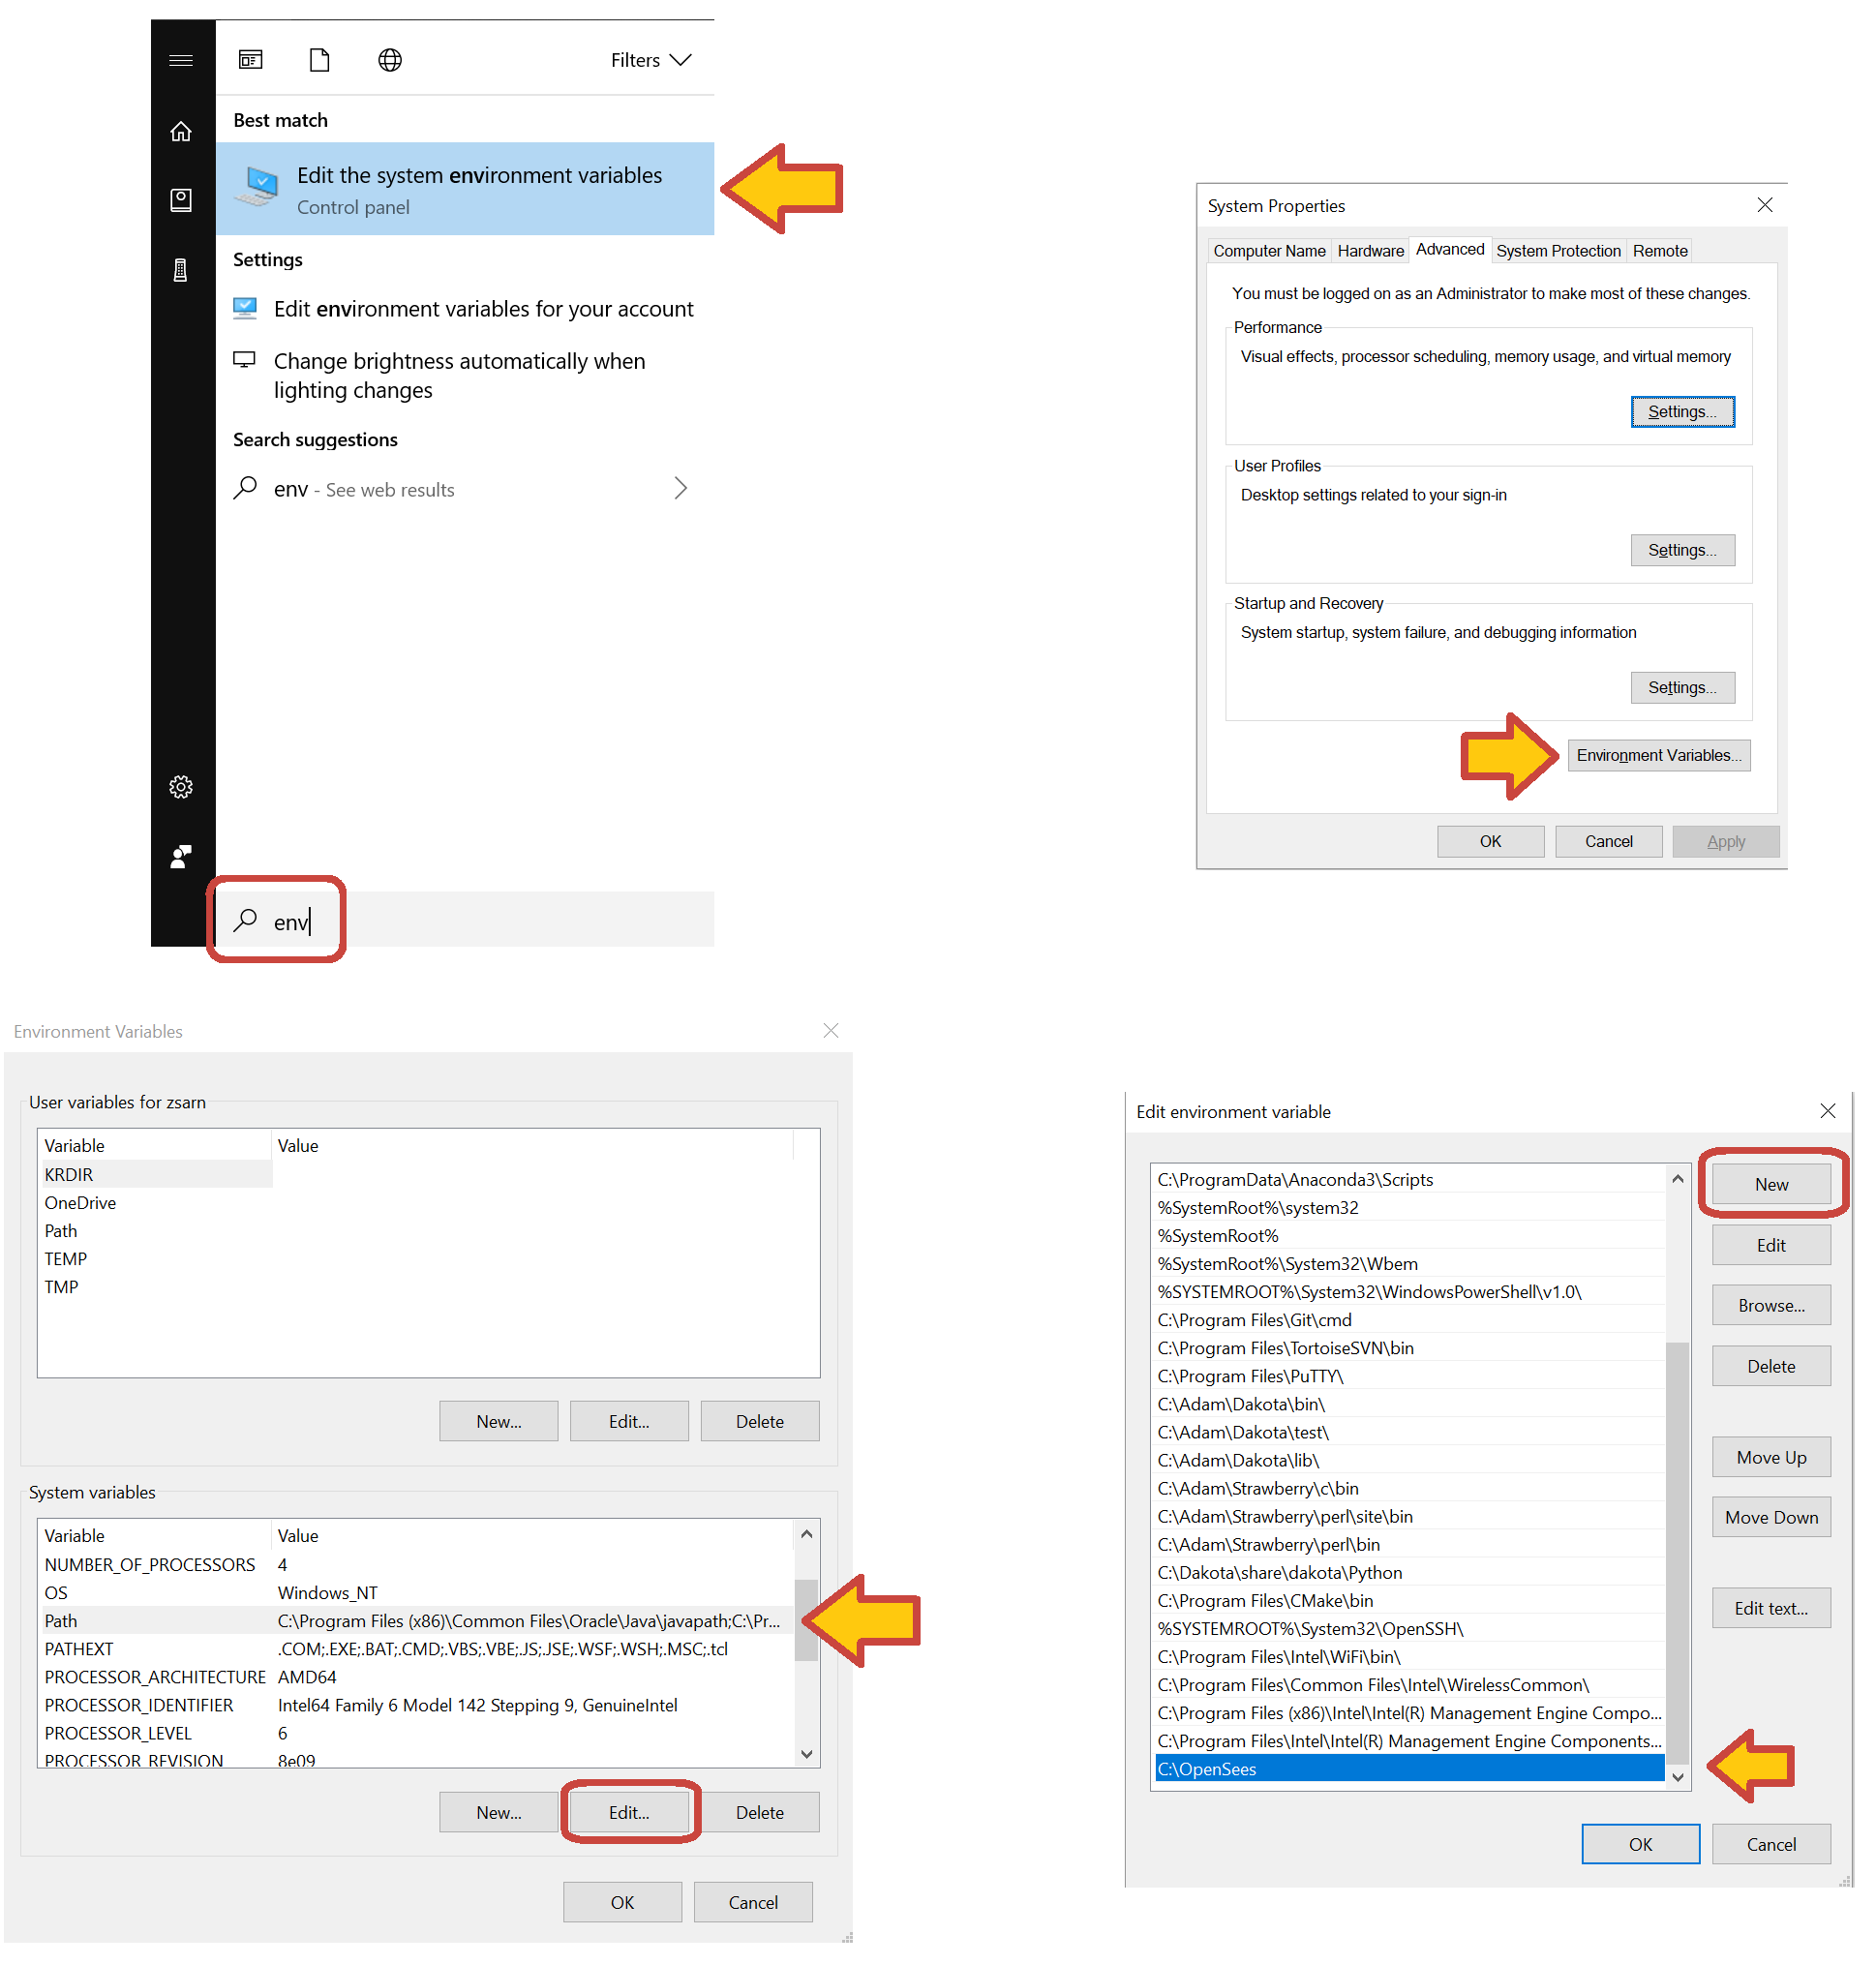
\includegraphics[width=0.8\textwidth]
    {figs/install/add_env_path.png} }
  \caption{Adding OpenSees to the PATH environment variable on Windows.}
  \label{fig:add_env_path}
\end{figure}

\begin{enumerate}
    \item open \emph{Start}, type \emph{env}, and choose \emph{Edit the system environment variables};
    \item click on the \emph{Environment variables...} button in the dialog window;
    \item find the \texttt{Path} under \emph{System Variables} in the \emph{Variable} column;
    \item click \emph{New} and type in the path to your \texttt{OpenSees.exe} (this will be \texttt{C:\\SimCenter\\OpenSees} if you put the executable at the recommended location - pay attention to using backward slashes here!);
    \item click \emph{OK} in every dialog to close them and save your changes.
\end{enumerate}

\item MacOS: To add the /usr/local/OpenSees folder to the \texttt{PATH} variable::

\begin{figure}[!htbp]
  \centering {
    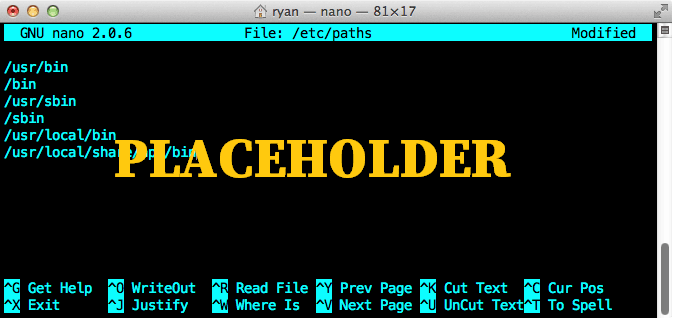
\includegraphics[width=0.8\textwidth]
    {figs/install/add_env_path_Mac.png} }
  \caption{Adding OpenSees to the PATH environment variable on Mac.}
  \label{fig:add_env_path_Mac}
\end{figure}

\begin{enumerate}
    \item open a Terminal;
    \item execute \texttt{sudo nano /etc/paths} and enter your password
    \item add the path to the OpenSees executable to the end of the list (this will be \texttt{/usr/local/OpenSees} if you put the executable at the recommended location);
    \item quit by hitting \texttt{Ctrl+X} and then \texttt{Y} when asked if you want to save modifications.
\end{enumerate}

\end{enumerate}



\subsection{Install Dakota}
%===============================================================================

\href{http://dakota.sandia.gov}{Dakota}, an open-source  optimization and UQ application from Sandia National Labs, is publicly available for download at its \href{http://dakota.sandia.gov/download.html}{download page}. Select your operating system from the list and set the other options as shown in  \autoref{fig:dakota_installation}. Download the release in a \texttt{ZIP} file for Windows and \texttt{TAR.GZ} file for Mac. We recommend you to extract the archive to a \texttt{C:/SimCenter/Dakota} folder on Windows, and to a \texttt{/usr/local/Dakota} folder on a Mac.

\begin{figure}[!htbp]
  \centering {
    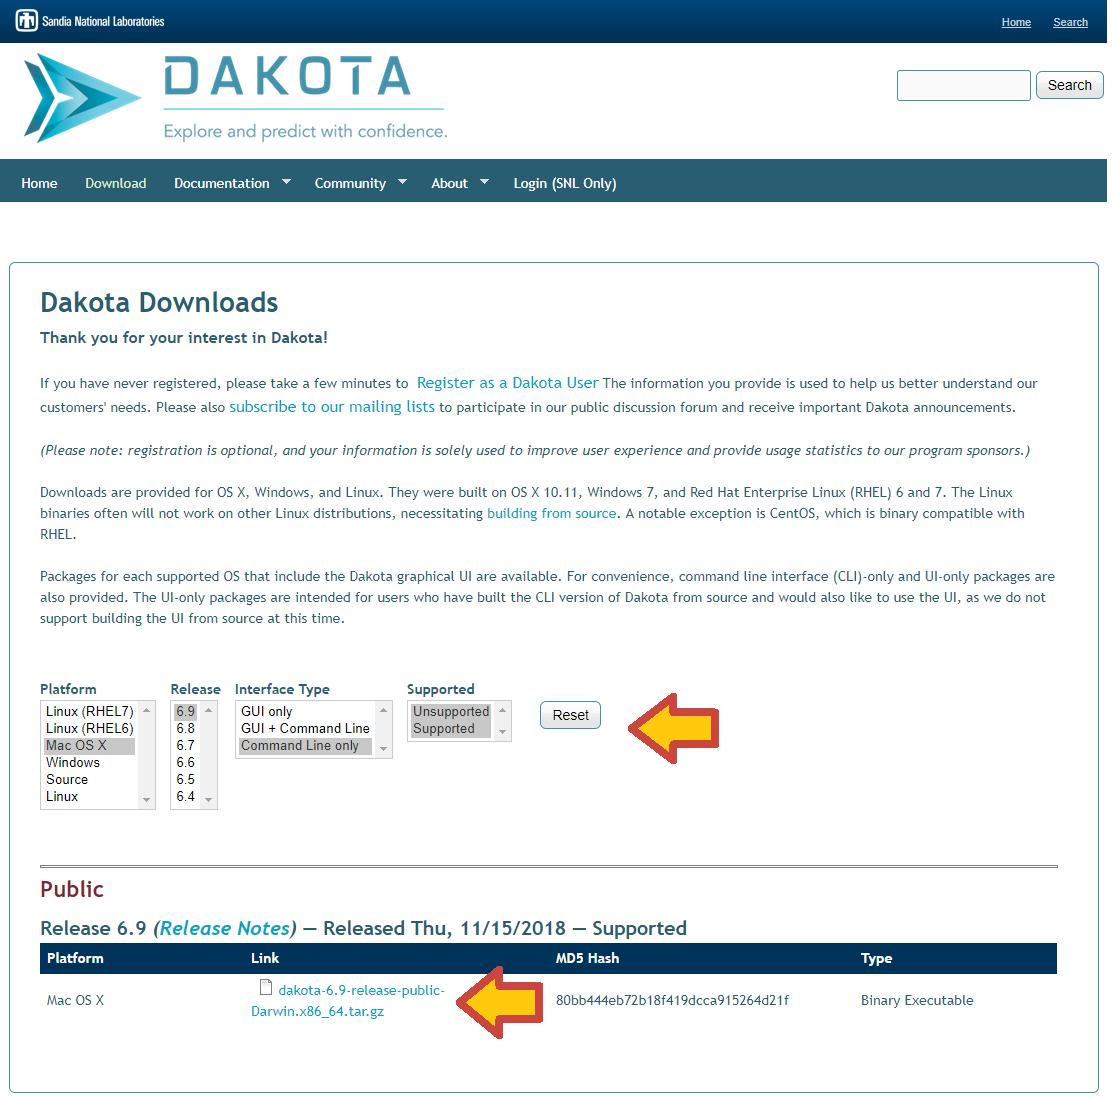
\includegraphics[width=0.8\textwidth]
    {figs/install/dakota_installation.png} }
  \caption{Adding OpenSees to the PATH environment variable on Mac.}
  \label{fig:dakota_installation}
\end{figure}

Similarly to OpenSees, you need to add TWO Dakota folders to the system \texttt{PATH} environment variable to allow the SimCenter workflow applications to find the Dakota tools on your computer. Use the procedure described above for OpenSees to add the following folders to your \texttt{PATH}:

\begin{enumerate}
\item Windows:
\begin{itemize}
    \item \texttt{C:\textbackslash SimCenter\textbackslash Dakota\textbackslash bin}
    \item \texttt{C:\textbackslash SimCenter\textbackslash Dakota\textbackslash share\textbackslash dakota\textbackslash Python}
\end{itemize}

\item MacOS:
\begin{itemize}
    \item \texttt{/usr/local/Dakota/bin}
    \item \texttt{/usr/local/Dakota/share/dakota/Python}
\end{itemize}
\end{enumerate}
\subsection{Install  Perl}
%===============================================================================

Mac OS X has Perl pre-installed, but Windows users will have to install it to be able to use  Dakota. We recommend you use Strawberry Perl; you can install it by downloading the executable from its \href{http://strawberryperl.com}{Strawberry Perl website} and running it.

\subsection{Test the Install of the Local Applications}
%===============================================================================

Before running the EE-UQ application, perform the following tests to make sure that the local SimCenter working environment is set up appropriately:

\begin{itemize}
    \item Start a Terminal on Mac or a Command Prompt on Windows.
    \item On Mac, execute \texttt{cd /usr/Documents} to change the active directory to \texttt{/usr/Documents}. On Windows, execute \texttt{cd C:/} to change the active directory to \texttt{C:/}.
    \item Test if OpenSees works correctly by executing the \texttt{OpenSees} command. The command should start OpenSees (\autoref{fig:opensees_test}). Close OpenSees with the \texttt{exit} command.
    \item Test if Dakota works correctly by executing the \texttt{dakota} command. The command should start Dakota and you should see a message about a missing argument (\autoref{fig:dakota_test}).
    \item Test if Perl works correctly by executing the \texttt{perl -v} command. The command should start Perl and return its version number (\autoref{fig:perl_test}).
    \item Test if the python package in Dakota works correctly by starting Python with the \texttt{python} command and then executing the \texttt{import dakota} command. This should import the dakota package. If you do not see errors, then the package is successfully imported (\autoref{fig:dakota_py_test}). Exit Python with the \texttt{exit()} command.
    \item If all the above tests ran without errors, your environment is set up appropriately.
\end{itemize}

\begin{figure}[!htbp]
  \centering {
    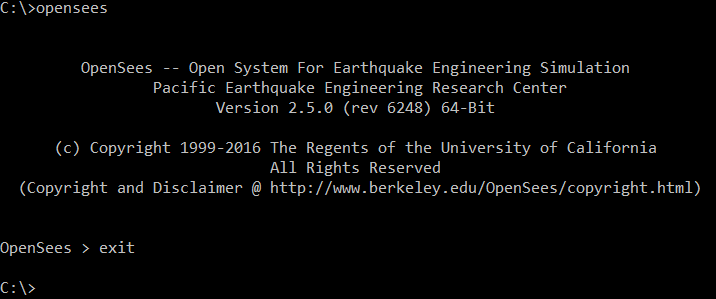
\includegraphics[width=0.8\textwidth]
    {figs/install/opensees_test.png} }
  \caption{Testing OpenSees.}
  \label{fig:opensees_test}
\end{figure}

\begin{figure}[!htbp]
  \centering {
    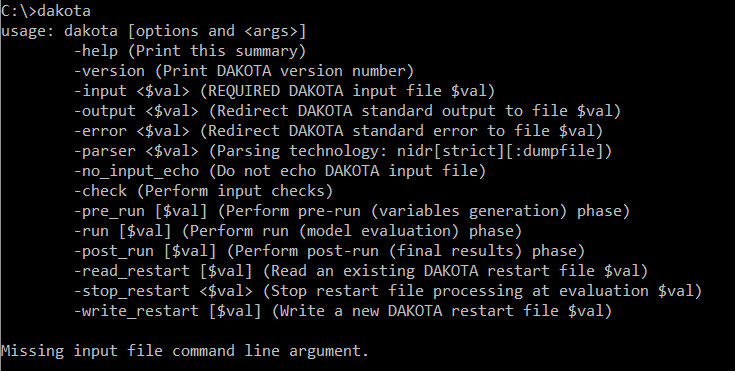
\includegraphics[width=0.8\textwidth]
    {figs/install/dakota_test.png} }
  \caption{Testing Dakota.}
  \label{fig:dakota_test}
\end{figure}

\begin{figure}[!htbp]
  \centering {
    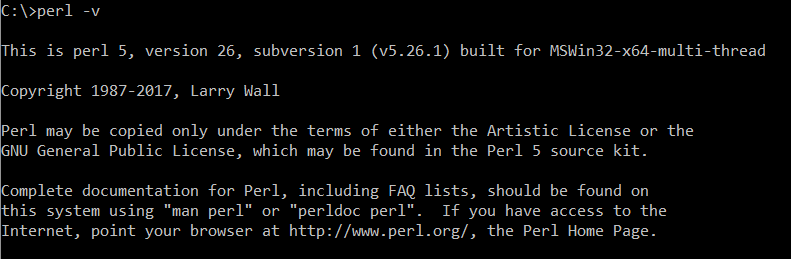
\includegraphics[width=0.8\textwidth]
    {figs/install/perl_test.png} }
  \caption{Testing Perl.}
  \label{fig:perl_test}
\end{figure}

\begin{figure}[!htbp]
  \centering {
    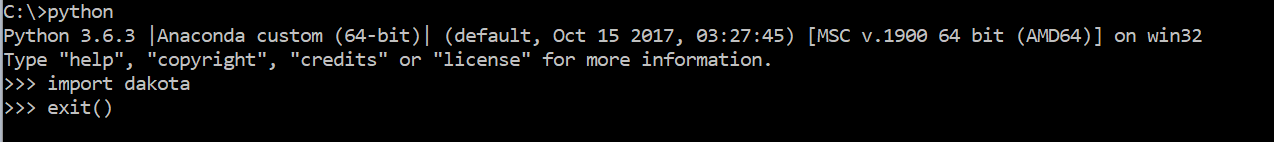
\includegraphics[width=0.8\textwidth]
    {figs/install/dakota_py_test.png} }
  \caption{Testing the dakota Python package.}
  \label{fig:dakota_py_test}
\end{figure}

%===============================================================================
\section{Test the EE-UQ application}\label{install_test}
%===============================================================================

\subsection{Run a remote calculation}
%===============================================================================

\subsection{Run a local calculation}
%===============================================================================

